\documentclass[a4paper]{article}

\def\npart {IB}
\def\nterm {Lent}
\def\nyear {2016}
\def\nlecturer {O. Randal-Williams}
\def\ncourse {Groups, Rings and Modules}
\def\nlectures {MWF.12}
\def\nnotready {}

% Imports
\ifx \nextra \undefined
  \usepackage[pdftex,
    hidelinks,
    pdfauthor={Dexter Chua},
    pdfsubject={Cambridge Maths Notes: Part \npart\ - \ncourse},
    pdftitle={Part \npart\ - \ncourse},
  pdfkeywords={Cambridge Mathematics Maths Math \npart\ \nterm\ \nyear\ \ncourse}]{hyperref}
  \title{Part \npart\ - \ncourse}
\else
  \usepackage[pdftex,
    hidelinks,
    pdfauthor={Dexter Chua},
    pdfsubject={Cambridge Maths Notes: Part \npart\ - \ncourse\ (\nextra)},
    pdftitle={Part \npart\ - \ncourse\ (\nextra)},
  pdfkeywords={Cambridge Mathematics Maths Math \npart\ \nterm\ \nyear\ \ncourse\ \nextra}]{hyperref}

  \title{Part \npart\ - \ncourse \\ {\Large \nextra}}
\fi

\author{Lectured by \nlecturer \\\small Notes taken by Dexter Chua}
\date{\nterm\ \nyear}

\usepackage{alltt}
\usepackage{amsfonts}
\usepackage{amsmath}
\usepackage{amssymb}
\usepackage{amsthm}
\usepackage{booktabs}
\usepackage{caption}
\usepackage{enumitem}
\usepackage{fancyhdr}
\usepackage{graphicx}
\usepackage{mathtools}
\usepackage{microtype}
\usepackage{multirow}
\usepackage{pdflscape}
\usepackage{pgfplots}
\usepackage{siunitx}
\usepackage{tabularx}
\usepackage{tikz}
\usepackage{tkz-euclide}
\usepackage[normalem]{ulem}
\usepackage[all]{xy}

\pgfplotsset{compat=1.12}

\pagestyle{fancyplain}
\lhead{\emph{\nouppercase{\leftmark}}}
\ifx \nextra \undefined
  \rhead{
    \ifnum\thepage=1
    \else
      \npart\ \ncourse
    \fi}
\else
  \rhead{
    \ifnum\thepage=1
    \else
      \npart\ \ncourse\ (\nextra)
    \fi}
\fi
\usetikzlibrary{arrows}
\usetikzlibrary{decorations.markings}
\usetikzlibrary{decorations.pathmorphing}
\usetikzlibrary{positioning}
\usetikzlibrary{fadings}
\usetikzlibrary{intersections}
\usetikzlibrary{cd}

\newcommand*{\Cdot}{\raisebox{-0.25ex}{\scalebox{1.5}{$\cdot$}}}
\newcommand {\pd}[2][ ]{
  \ifx #1 { }
    \frac{\partial}{\partial #2}
  \else
    \frac{\partial^{#1}}{\partial #2^{#1}}
  \fi
}

% Theorems
\theoremstyle{definition}
\newtheorem*{aim}{Aim}
\newtheorem*{axiom}{Axiom}
\newtheorem*{claim}{Claim}
\newtheorem*{cor}{Corollary}
\newtheorem*{defi}{Definition}
\newtheorem*{eg}{Example}
\newtheorem*{fact}{Fact}
\newtheorem*{law}{Law}
\newtheorem*{lemma}{Lemma}
\newtheorem*{notation}{Notation}
\newtheorem*{prop}{Proposition}
\newtheorem*{thm}{Theorem}

\renewcommand{\labelitemi}{--}
\renewcommand{\labelitemii}{$\circ$}
\renewcommand{\labelenumi}{(\roman{*})}

\let\stdsection\section
\renewcommand\section{\newpage\stdsection}

% Strike through
\def\st{\bgroup \ULdepth=-.55ex \ULset}

% Maths symbols
\newcommand{\bra}{\langle}
\newcommand{\ket}{\rangle}

\newcommand{\N}{\mathbb{N}}
\newcommand{\Z}{\mathbb{Z}}
\newcommand{\Q}{\mathbb{Q}}
\renewcommand{\H}{\mathbb{H}}
\newcommand{\R}{\mathbb{R}}
\newcommand{\C}{\mathbb{C}}
\newcommand{\Prob}{\mathbb{P}}
\renewcommand{\P}{\mathbb{P}}
\newcommand{\E}{\mathbb{E}}
\newcommand{\F}{\mathbb{F}}
\newcommand{\cU}{\mathcal{U}}
\newcommand{\RP}{\mathbb{RP}}
\newcommand{\CP}{\mathbb{CP}}

\newcommand{\ph}{\,\cdot\,}

\DeclareMathOperator{\sech}{sech}
\DeclareMathOperator{\cosech}{cosech}
\DeclareMathOperator{\cosec}{cosec}

\DeclareMathOperator{\covol}{covol}
\DeclareMathOperator{\vol}{vol}

\let\Im\relax
\let\Re\relax
\DeclareMathOperator{\Im}{Im}
\DeclareMathOperator{\Re}{Re}
\DeclareMathOperator{\im}{im}
\DeclareMathOperator{\image}{image}
\DeclareMathOperator{\Ann}{Ann}

\DeclareMathOperator*{\res}{res}
\DeclareMathOperator{\Res}{Res}
\DeclareMathOperator{\Ind}{Ind}

\DeclareMathOperator{\tr}{tr}
\DeclareMathOperator{\diag}{diag}
\DeclareMathOperator{\rank}{rank}
\DeclareMathOperator{\card}{card}
\DeclareMathOperator{\spn}{span}
\DeclareMathOperator{\adj}{adj}

\DeclareMathOperator{\erf}{erf}
\DeclareMathOperator{\erfc}{erfc}

\DeclareMathOperator{\ord}{ord}
\DeclareMathOperator{\Sym}{Sym}

\DeclareMathOperator{\sgn}{sgn}
\DeclareMathOperator{\orb}{orb}
\DeclareMathOperator{\stab}{stab}
\DeclareMathOperator{\ccl}{ccl}

\DeclareMathOperator{\lcm}{lcm}
\DeclareMathOperator{\hcf}{hcf}

\DeclareMathOperator{\Int}{Int}
\DeclareMathOperator{\id}{id}

\DeclareMathOperator{\betaD}{beta}
\DeclareMathOperator{\gammaD}{gamma}
\DeclareMathOperator{\Poisson}{Poisson}
\DeclareMathOperator{\binomial}{binomial}
\DeclareMathOperator{\multinomial}{multinomial}
\DeclareMathOperator{\Bernoulli}{Bernoulli}
\DeclareMathOperator{\like}{like}

\DeclareMathOperator{\var}{var}
\DeclareMathOperator{\cov}{cov}
\DeclareMathOperator{\bias}{bias}
\DeclareMathOperator{\mse}{mse}
\DeclareMathOperator{\corr}{corr}

\DeclareMathOperator{\otp}{otp}
\DeclareMathOperator{\dom}{dom}

\DeclareMathOperator{\Root}{Root}
\DeclareMathOperator{\supp}{supp}
\DeclareMathOperator{\rel}{rel}
\DeclareMathOperator{\Hom}{Hom}
\DeclareMathOperator{\Aut}{Aut}
\DeclareMathOperator{\Gal}{Gal}
\DeclareMathOperator{\Mat}{Mat}
\DeclareMathOperator{\End}{End}
\DeclareMathOperator{\Char}{char}
\DeclareMathOperator{\ev}{ev}
\DeclareMathOperator{\St}{St}
\DeclareMathOperator{\Lk}{Lk}
\DeclareMathOperator{\disc}{disc}
\DeclareMathOperator{\Isom}{Isom}
\DeclareMathOperator{\length}{length}
\DeclareMathOperator{\energy}{energy}
\DeclareMathOperator{\area}{area}
\DeclareMathOperator{\Syl}{Syl}
\DeclareMathOperator{\cl}{cl}
\DeclareMathOperator{\fix}{fix}

\newcommand{\GL}{\mathrm{GL}}
\newcommand{\SL}{\mathrm{SL}}
\newcommand{\PGL}{\mathrm{PGL}}
\newcommand{\PSL}{\mathrm{PSL}}
\newcommand{\PSU}{\mathrm{PSU}}
\newcommand{\Or}{\mathrm{O}}
\newcommand{\SO}{\mathrm{SO}}
\newcommand{\U}{\mathrm{U}}
\newcommand{\SU}{\mathrm{SU}}

\renewcommand{\d}{\mathrm{d}}
\newcommand{\D}{\mathrm{D}}

\tikzset{->/.style = {decoration={markings,
                                  mark=at position 1 with {\arrow[scale=2]{latex'}}},
                      postaction={decorate}}}
\tikzset{<-/.style = {decoration={markings,
                                  mark=at position 0 with {\arrowreversed[scale=2]{latex'}}},
                      postaction={decorate}}}
\tikzset{<->/.style = {decoration={markings,
                                   mark=at position 0 with {\arrowreversed[scale=2]{latex'}},
                                   mark=at position 1 with {\arrow[scale=2]{latex'}}},
                       postaction={decorate}}}
\tikzset{->-/.style = {decoration={markings,
                                   mark=at position #1 with {\arrow[scale=2]{latex'}}},
                       postaction={decorate}}}
\tikzset{-<-/.style = {decoration={markings,
                                   mark=at position #1 with {\arrowreversed[scale=2]{latex'}}},
                       postaction={decorate}}}

\tikzset{circ/.style = {fill, circle, inner sep = 0, minimum size = 3}}
\tikzset{mstate/.style={circle, draw, blue, text=black, minimum width=0.7cm}}

\definecolor{mblue}{rgb}{0.2, 0.3, 0.8}
\definecolor{morange}{rgb}{1, 0.5, 0}
\definecolor{mgreen}{rgb}{0.1, 0.4, 0.2}
\definecolor{mred}{rgb}{0.5, 0, 0}

\def\drawcirculararc(#1,#2)(#3,#4)(#5,#6){%
    \pgfmathsetmacro\cA{(#1*#1+#2*#2-#3*#3-#4*#4)/2}%
    \pgfmathsetmacro\cB{(#1*#1+#2*#2-#5*#5-#6*#6)/2}%
    \pgfmathsetmacro\cy{(\cB*(#1-#3)-\cA*(#1-#5))/%
                        ((#2-#6)*(#1-#3)-(#2-#4)*(#1-#5))}%
    \pgfmathsetmacro\cx{(\cA-\cy*(#2-#4))/(#1-#3)}%
    \pgfmathsetmacro\cr{sqrt((#1-\cx)*(#1-\cx)+(#2-\cy)*(#2-\cy))}%
    \pgfmathsetmacro\cA{atan2(#2-\cy,#1-\cx)}%
    \pgfmathsetmacro\cB{atan2(#6-\cy,#5-\cx)}%
    \pgfmathparse{\cB<\cA}%
    \ifnum\pgfmathresult=1
        \pgfmathsetmacro\cB{\cB+360}%
    \fi
    \draw (#1,#2) arc (\cA:\cB:\cr);%
}
\newcommand\getCoord[3]{\newdimen{#1}\newdimen{#2}\pgfextractx{#1}{\pgfpointanchor{#3}{center}}\pgfextracty{#2}{\pgfpointanchor{#3}{center}}}

\def\Xint#1{\mathchoice
   {\XXint\displaystyle\textstyle{#1}}%
   {\XXint\textstyle\scriptstyle{#1}}%
   {\XXint\scriptstyle\scriptscriptstyle{#1}}%
   {\XXint\scriptscriptstyle\scriptscriptstyle{#1}}%
   \!\int}
\def\XXint#1#2#3{{\setbox0=\hbox{$#1{#2#3}{\int}$}
     \vcenter{\hbox{$#2#3$}}\kern-.5\wd0}}
\def\ddashint{\Xint=}
\def\dashint{\Xint-}


\begin{document}
\maketitle
{\small
\noindent\textbf{Groups}\\
Basic concepts of group theory recalled from Part IA Groups. Normal subgroups, quotient groups and isomorphism theorems. Permutation groups. Groups acting on sets, permutation representations. Conjugacy classes, centralizers and normalizers. The centre of a group. Elementary properties of finite $p$-groups. Examples of finite linear groups and groups arising from geometry. Simplicity of $A_n$.

\vspace{5pt}
\noindent Sylow subgroups and Sylow theorems. Applications, groups of small order.\hspace*{\fill} [8]

\vspace{10pt}
\noindent\textbf{Rings}\\
Definition and examples of rings (commutative, with 1). Ideals, homomorphisms, quotient rings, isomorphism theorems. Prime and maximal ideals. Fields. The characteristic of a field. Field of fractions of an integral domain.

\vspace{5pt}
\noindent Factorization in rings; units, primes and irreducibles. Unique factorization in principal ideal domains, and in polynomial rings. Gauss' Lemma and Eisenstein's irreducibility criterion.

\vspace{5pt}
\noindent Rings $\Z[\alpha]$ of algebraic integers as subsets of $\C$ and quotients of $\Z[x]$. Examples of Euclidean domains and uniqueness and non-uniqueness of factorization. Factorization in the ring of Gaussian integers; representation of integers as sums of two squares.

\vspace{5pt}
\noindent Ideals in polynomial rings. Hilbert basis theorem.\hspace*{\fill} [10]

\vspace{10pt}
\noindent\textbf{Modules}\\
Definitions, examples of vector spaces, abelian groups and vector spaces with an endomorphism. Sub-modules, homomorphisms, quotient modules and direct sums. Equivalence of matrices, canonical form. Structure of finitely generated modules over Euclidean domains, applications to abelian groups and Jordan normal form.\hspace*{\fill} [6]}

\tableofcontents

\section{Groups}
\subsection{Basic concepts}
\begin{defi}[Group]
  A \emph{group} is a triple $(G, \ph, e)$, where $G$ is a set, $\ph: G\times G \to G$ is a function and $e \in G$ such that
  \begin{enumerate}
    \item For all $a, b, c \in G$, $(a \cdot b) \cdot c = a \cdot (b \cdot c)$.\hfill (associativity)
    \item For all $a \in G$, $a \cdot e = e \cdot a = a$.\hfill (identity)
    \item For all $a \in G$, there exists $a^{-1} \in G$ such that $a \cdot a^{-1} = a^{-1} \cdot a = e$.\hfill (inverse)
  \end{enumerate}
\end{defi}
Some people add a stupid axiom that $g \cdot h \in G$ for all $g, h \in G$, but this is already implied by saying $\cdot$ is a function to $G$. You can write that down as well, and no one will say you are stupid. But they might \emph{think} so.

\begin{lemma}
  The inverse of an element is unique.
\end{lemma}

\begin{proof}
  Let $a^{-1}, b$ be inverses of $a$. Then
  \[
    b = b \cdot e = b \cdot a \cdot a^{-1} = e \cdot a^{-1} = a^{-1}.
  \]
\end{proof}

\begin{defi}[Subgroup]
  If $(G, \ph)$ is a group and $H \subseteq G$ is a subset, it is a \emph{subgroup} if
  \begin{enumerate}
    \item $e \in H$,
    \item $a, b \in H$ implies $a\cdot b\in H$,
    \item $\ph: H \times H \to H$ makes $(H, \ph, e)$ a group.
  \end{enumerate}
  We write $H \leq G$ if $H$ is a subgroup of $G$.
\end{defi}
Note that the last condition in some sense encompasses the first two, but we need the first two conditions to hold before that statement makes sense at all.

\begin{lemma}
  $H \subseteq G$ is a subgroup if $H$ is non-empty and for any $h_1, h_2 \in H$, we have $h_1h_2^{-1} \in H$.
\end{lemma}

\begin{defi}[Abelian group]
  A group $G$ is \emph{abelian} if $a\cdot b = b\cdot a$ for all $a, b\in G$.
\end{defi}

\begin{eg}\leavevmode
  \begin{enumerate}
    \item The following are groups: $(\Z, +, 0)$, $(\Q, +, 0)$, $(\R, +, 0)$, $(\C, +, 0)$.
    \item Groups of symmetries
      \begin{enumerate}
        \item The symmetric group $S_n$ of permutations of $\{1, 2, \cdots, n\}$.
        \item The dihedral group $D_{2n}$ is the symmetries of a regular $n$-gon.
        \item The group $\GL_n(\R)$ is the group of invertible $n\times n$ real matrices, which also is the group of invertible $\R$-linear maps from the vector space $\R^n$ to itself.
      \end{enumerate}
    \item The alternating group $A_n \leq S_n$.
    \item The cyclic group $C_n \leq D_{2n}$.
    \item The special linear group $\SL_n(\R) \leq \GL_n(\R)$, the subgroup of matrices of determinant $1$.
    \item The Klein-four group $C_2 \times C_2$.
    \item The quaternions $Q_8 = \{\pm 1, \pm i, \pm j, \pm k\}$ with $ij = k, ji = -k$, $i^2 = j^2 = k^2 = -1$, $(-1)^2 = 1$.
  \end{enumerate}
\end{eg}

With groups and subgroups, we can talk about cosets.
\begin{defi}[Coset]
  If $H \leq G$, $g \in G$, the \emph{left coset} $gH$ is the set
  \[
    gH = \{x \in G: x = g\cdot h\text{ for some }h \in H\}.
  \]
\end{defi}
For example, since $H$ is a subgroup, we know $e \in H$. So for any $g \in G$, we must have $g \in gH$.

The collection of $H$-cosets in $G$ forms a partition of $G$, and furthermore, all $H$ cosets $gH$ are in bijection with $H$ itself, via $h \mapsto gh$. An immediate consequence is
\begin{thm}[Lagrange's theorem]
  Let $G$ be a finite group, and $H \leq G$. Then
  \[
    |G| = |H| |G:H|,
  \]
  where $|G:H|$ is the number of $H$ cosets in $G$.
\end{thm}
We can do exactly the same thing with right cosets and get the same conclusion.

We have implicitly used the following notation:
\begin{defi}[Order of group]
  The \emph{order} of a group is the number of elements in $G$, written $|G|$.
\end{defi}

Instead of order of the group, we can ask what the order of an element is.
\begin{defi}[Order of element]
  The \emph{order} of an element $g \in G$ is the smallest positive $n$ such that $g^n = e$. If there is no such $n$, we say $g$ has infinite order.

  We write $\ord(g) = n$.
\end{defi}

A basic lemma is as follows:
\begin{lemma}
  If $G$ is a finite group and $g \in G$ has order $n$, then $n \mid G$.
\end{lemma}

\begin{proof}
  Consider the following subset:
  \[
    H= \{e, g, g^2, \cdots, g^{n - 1}\}.
  \]
  This is a subgroup of $G$, because it is non-empty and $g^rg^{-s} = g^{r - s}$ is on the list (we might have to add $n$ to the power of $g$ to make it positive, but this is fine since $g^n = e$). Moreover, there are no repeats in the list: if $g^i = g^j$, with wlog $i \geq j$, then $g^{i - j} = e$. So $i - j < n$. By definition of $n$, we must have $i - j = 0$, ie. $i = j$.

  Hence Lagrange's theorem tells us $n = |H| \mid |G|$.
\end{proof}

\subsection{Normal subgroups, quotients, homomorphisms, isomorphisms}
We all know what the definition of a normal subgroup is. But if we were not given the definition, how could we have come up with it?

Let $H \leq G$ be a subgroup. Notice that if $gH = g'H$, then $g \in g'H$. So $g = g'\cdot h$ for some $h$. In other words, $(g')^{-1} \cdot g = h \in H$. So if two elements represent the same coset, their difference is in $H$. The argument is also reversible. Hence two elements $g, g'$ represent the same $H$-coset if and only if $(g')^{-1} g \in H$.

Suppose we try to make the set $G/H = \{gH: g \in G\}$ into a group, by the obvious formula
\[
  (g_1 H) \cdot (g_2 H) = g_1 g_2 H.
\]
However, this doesn't necessarily make sense. If we take a different representative for the same coset, we want to make sure it gives the same answer. If $g_2 H = g_2' H$, then $g_2' = g_2 \cdot h$ for some $h \in H$. So
\[
  (g_1 H) \cdot (g_2' H) = g_1 g_2' H = g_1 g_2 h H = g_1g_2 H = (g_1 H) \cdot (g_2 H).
\]
So all is good.

What if we change $g_1$? If $g_1H = g_1' H$, then $g_1' = g_1 \cdot h$ for some $h \in H$. So
\[
  (g_1' H) \cdot (g_2 H) = g_1' g_2 H = g_1 h g_2 H.
\]
Now we are stuck. We would really want the equality
\[
  g_1 h g_2 H = g_1 g_2 H
\]
to hold. This requires
\[
  (g_1g_2)^{-1} g_1 h g_2 \in H.
\]
This is equivalent to
\[
  g_2^{-1} h g_2 \in H.
\]
So for $G/H$ to actually be a group under this operation, we must have, for any $h \in H$ and $g \in G$, the property $g^{-1} h g \in H$ to hold.

This is not necessarily true for an arbitrary $H$. Those nice ones that satisfy this property are known as \emph{normal subgroups}.
\begin{defi}[Normal subgroup]
  A subgroup $H \leq G$ is \emph{normal} if for any $h \in H$ and $g \in G$, we have $g^{-1}h g \in H$. We write $H \lhd G$.
\end{defi}

This allows us to make the following definition:
\begin{defi}[Quotient group]
  If $H \lhd G$ is a normal subgroup, then the set $G/H$ of left $H$-cosets forms a group with multiplication
  \[
    (g_1 H) \cdot (g_2 H) = g_1 g_2 H.
  \]
  with identity $eH = H$. This is known as the \emph{quotient group}.
\end{defi}
This is indeed a group. Normality was defined such that this is well-defined. Multiplication is associative since multiplication in $G$ is associative. The inverse of $gH$ is $g^{-1}H$, and $eH$ is easily seen to be the identity.

So far, we've just been looking at groups themselves. We would also like to know how groups interact with each other. In other words, we want to study functions between groups. However, we don't allow \emph{arbitrary} functions, since groups have some structure, and we would like the functions to respect the group structures. These nice functions are known as \emph{homomorphisms}.

\begin{defi}[Homomorphism]
  If $(G, \ph, e_G)$ and $(H, *, e_H)$ are groups, a function $\phi: G\to H$ is a \emph{homomorphism} if $\phi(e_G) = e_H$, and for $g, g' \in G$, we have
  \[
    \phi(g \cdot g') = \phi(g) * \phi(g').
  \]
\end{defi}
If we think carefully, $\phi(e_G) = e_H$ can be derived from the second condition, but we could as well put it in as well. It is easy to show the following:
\begin{lemma}
  If $\phi: G \to H$ is a homomorphism, then
  \[
    \phi(g^{-1}) = \phi(g)^{-1}.
  \]
\end{lemma}

\begin{proof}
  We compute $\phi(g\cdot g^{-1})$ in two ways. On the one hand, we have
  \[
    \phi(g\cdot g^{-1}) = \phi(e) = e.
  \]
  On the other hand, we have
  \[
    \phi(g\cdot g^{-1}) = \phi(g) * \phi(g^{-1}).
  \]
  By the uniqueness of inverse, we must have
  \[
    \phi(g^{-1}) = \phi(g)^{-1}.
  \]
\end{proof}

Given any homomorphism, we can build two groups out of it:
\begin{defi}[Kernel]
  The \emph{kernel} of a homomorphism $\phi: G \to H$ is
  \[
    \ker(\phi) = \{g \in G: \phi(g) = 0\}.
  \]
\end{defi}

\begin{defi}[Image]
  The \emph{image} of a homomorphism $\phi: G \to H$ is
  \[
    \im (\phi) = \{h\in H: h = \phi(g) \text{ for some }g \in G\}.
  \]
\end{defi}

There are some basic properties about these:
\begin{lemma}
  For a homomorphism $\phi: G\to H$, the kernel $\ker (\phi)$ is a \emph{normal subgroup}, and the image $\im (\phi)$ is a subgroup of $H$.
\end{lemma}

There is only one possible way we can prove this.
\begin{proof}
  To see $\ker(\phi)$ is a subgroup, let $g, h \in \ker \phi$. Then
  \[
    \phi(g\cdot h^{-1}) = \phi(g) * \phi(h)^{-1} = e * e^{-1} = e.
  \]
  So $gh^{-1} \in \ker \phi$. Also, $\phi(e) = e$. So $\ker(\phi)$ is non-empty. So it is a subgroup.

  To show it is normal, let $g \in \ker(\phi)$. Let $x \in G$. we want to show $x^{-1}gx \in \ker(\phi)$. We have
  \[
    \phi(x^{-1} xg) = \phi(x^{-1}) * \phi(g) * \phi(x) = \phi(x^{-1}) * \phi(x) = \phi(x^{-1}x) = \phi(e) = e.
  \]
  So $x^{-1}gx \in \ker(\phi)$. So $\ker(\phi)$ is normal.

  Also, if $\phi(g), \phi(h) \in \im (\phi)$, then
  \[
    \phi(g) * \phi(h)^{-1} = \phi(gh^{-1}) \in \im (\phi).
  \]
  Also, $e \in \im(\phi)$. So $\im(\phi)$ is a subgroup.
\end{proof}

Homomorphisms are nice. But those that are bijections are even nicer.
\begin{defi}[Isomorphism]
  An \emph{isomorphism} is a homomorphism that is also a bijection.
\end{defi}

\begin{defi}[Isomorphic group]
  Two groups $G$ and $H$ are \emph{isomorphic} if there is an isomorphism between them. We write $G \cong H$.
\end{defi}
Usually, we identify two isomorphic groups as being ``the same''.

It is an exercise to show the following:
\begin{lemma}
  If $\phi$ is an isomorphism, then the inverse $\phi^{-1}$ is also an isomorphism.
\end{lemma}

When studying groups, it is often helpful to break the group apart into smaller groups, which are hopefully easier to study. We will have three isomorphism theorems to do so. These allow us to break our groups apart into smaller groups, and then if a miracle happens, we can patch these together to get information about the big group. Even if miracles do not happen, these are useful tools to have.

% complete

An important theorem relating the image and the kernel of a homomorphism is the following:
\begin{thm}[First isomorphism theorem]
  Let $\phi: G \to H$ is a homomorphism, then $\ker(\phi) \lhd G$ and
  \[
    \frac{G}{\ker (\phi)} \cong \im (\phi).
  \]
\end{thm}

\begin{proof}
  We have already proved that $\ker (\phi)$ is a normal subgroup. We now have to construct a homomorphism $\phi: G/\ker(\phi) \to \im (\phi)$, and prove it is an isomorphism.

  Define our function as follows:
  \begin{align*}
    f: \frac{G}{\ker (\phi)} &\to \im (\phi)\\
    g\ker (\phi) &\mapsto \phi(g).
  \end{align*}
  We first tackle the obvious problem that this might not be well-defined, since we are picking a representative for the coset. If $g \ker(\phi) = g' \ker(\phi)$, then we know $g^{-1} \cdot g' \in \ker(\phi)$. So $\phi(g^{-1} \cdot g') = e$. So we know
  \[
    e = \phi(g^{-1} \cdot g') = \phi(g)^{-1} * \phi(g').
  \]
  Multiplying the whole thing by $\phi(g)$ gives $\phi(g) = \phi(g')$. Hence this function is well-defined.

  Next we show it is a homomorphism. To see $f$ is a homomorphism, we have
  \begin{align*}
    f(g\ker (\phi) \cdot g'\ker(\phi)) &= f(gg'\ker(\phi)) \\
    &= \phi(gg') \\
    &= \phi(g) * \phi(g') \\
    &= f(g\ker(\phi)) * f(g'\ker(\phi)).
  \end{align*}
  So $f$ is a homomorphism. Finally, we show it is a bijection.

  To show it is surjective, let $h \in \im (\phi)$. Then $h = \phi(g)$ for some $g$. So $h = f(g\ker (\phi))$ is in the image of $f$.

  To show injectivity, suppose $f(g\ker (\phi)) = f(g'\ker(\phi))$. So $\phi(g) = \phi(g')$. So $\phi(g^{-1} \cdot g') = e$. Hence $g^{-1} \cdot g' \in \ker(\phi)$, and hence $g \ker(\phi) = g'\ker(\phi)$. So done.
\end{proof}

Before we move on to further isomorphism theorems, we see how we can use these to identify two groups which are not obvious the same.

\begin{eg}
  Consider a homomorphism $\phi: \C \to \C\setminus \{0\}$ given by $z \mapsto e^z$. We also know that
  \[
    e^{z + w} = e^z e^w.
  \]
  This means $\phi$ is a homomorphism if we think of it as $\phi: (\C, +) \to (\C\setminus \{0\}, \times)$.

  What is the image of this homomorphism? The existence of $\log$ shows that $\phi$ is surjective. So $\im \phi = \C\setminus \{0\}$. What about the kernel? It is given by
  \[
    \ker(\phi) = \{z \in \C: e^z = 1\} = 2\pi i \Z,
  \]
  ie. the set of all integer multiples of $2\pi i$. The conclusion is that
  \[
    (\C / (2\pi i \Z), +) \cong (\C\setminus \{0\}, \times).
  \]
\end{eg}

The second isomorphism is a slightly more complicated theorem.
\begin{thm}[Second isomorphism theorem]
  Let $H \leq G$ and $K \lhd G$. Then $HK = \{h\cdot k: h \in H, k \in K\}$ is a subgroup of $G$, and $H\cap K \lhd H$. Moreover,
  \[
    \frac{HK}{K} \cong \frac{H}{H \cap K}.
  \]
\end{thm}

\begin{proof}
  Let $hk, h'k' \in HK$. Then
  \[
    h'k'(hk)^{-1} = h'k' k^{-1}h^{-1} = (h'h^{-1})(hk'k^{-1}h^{-1}).
  \]
  The first term is in $H$, while the second term is $k'k^{-1} \in K$ conjugated by $h$, which also has to be in $K$ be normality. So this is something in $H$ times something in $K$, and hence in $HK$. $HK$ also contains $e$, and is hence a group.

  To show $H \cap K \lhd H$, consider $x \in H\cap K$ and $h \in H$. Consider $h^{-1} x h$. Since $x \in K$, the normality of $K$ implies $h^{-1}xh \in K$. Also, since $x, h \in H$, closure implies $h^{-1}xh \in H$. So $h^{-1} x h \in H \cap K$. So $H \cap K \lhd H$.

  Now we can start to prove the second isomorphism theorem. To do so, we apply the first isomorphism theorem to it. Define
  \begin{align*}
    \phi: H &\to G/K\\
    &h \mapsto hK
  \end{align*}
  This is easily seen to be a homomorphism. We apply the first isomorphism theorem to this homomorphism. The image is all $K$ cosets represented by something in $H$, ie.
  \[
    \im (\phi) = \frac{HK}{K}.
  \]
  Then the kernel of $\phi$ is
  \[
    \ker(\phi) = \{h: hK = eK\} = \{h: h \in K\} = H \cap K.
  \]
  So the first isomorphism theorem says
  \[
    \frac{H}{H \cap K} = \frac{HK}{K}.
  \]
\end{proof}
Notice we did more work than we really had to. We could have started by writing down $\phi$ and checked it is a homomorphism. Then since $H \cap K$ is its kernel, it has to be a normal subgroup.

Before we move on to the third isomorphism theorem, we notice that if $K \lhd G$, then there is a bijection
\begin{align*}
  \{\text{subgroups of }G/K\} &\longleftrightarrow\{\text{subgroups of }G\text{ which contain }K\}\\
  X \leq \frac{G}{K} &\longrightarrow \{g \in G: gK \in X\}\\
  \frac{L}{K} \leq \frac{G}{K} &\longleftarrow K \lhd L \leq G.
\end{align*}
It is an elementary exercise to show that these are inverses of each other.

This specializes to the bijection of normal subgorups:
\[
  \{\text{normal subgroups of }G/K\} \longleftrightarrow\{\text{normal subgroups of }G\text{ which contain }K\}\\
\]
using the same bijection.

\begin{thm}[Third isomorphism theorem]
  Let $K \leq L \leq G$ be normal subgroups of $G$. Then
  \[
    \frac{G}{K}\big/ \frac{L}{K} \cong \frac{G}{L}.
  \]
\end{thm}

\begin{proof}
  Define the homomorphism
  \begin{align*}
    \phi: G/K &\to G/L\\
    gK &\mapsto gL
  \end{align*}
  As always, we have to check this is well-defined. If $gK = g'K$, then $g^{-1}g' \in K \subseteq L$. So $gL = g'L$. This is also a homomorphism since
  \[
    \phi(gK \cdot g'K) = \phi(gg'K) = gg'L = (gL) \cdot (g'L) = \phi(gK) \cdot \phi(g'K).
  \]
  This clearly is surjective, since any coset $gL$ is the image $\phi(gK)$. So the image is $G/L$. The kernel is then
  \[
    \ker(\phi) = \{gK: gL = L\} = \{gK: g \in L\} = \frac{L}{K}.
  \]
  So the conclusion follows by the first isomorphism theorem.
\end{proof}

The general idea of these theorems is to take a group, find a normal subgroup, and then quotient it out. Then hopefully the normal subgorup and the quotient group will be simpler. However, this doesn't always work.

\begin{defi}[Simple group]
  A (non-trivial) group $G$ is \emph{simple} if it has no normal subgroups except $\{e\}$ and $G$.
\end{defi}

\begin{lemma}
  An abelian group is simple if and only if it is isomorphic to the cyclic group $C_p$ for some prime number $p$.
\end{lemma}

\begin{proof}
  By Lagrange's theorem, any subgruop of $C_p$ has order dividing $|C_p| = p$. Hence if $p$ is prime, then it has no such divisors, and any subgroup must have order $1$ or $p$, ie. it is either $\{e\}$ or $C_p$ itself. Hence in particular any normal subgroup must be $\{e\}$ or $C_p$. So it is simple.

  Now suppose $G$ is abelian and simple. Let $e \not= g \in G$ be a non-trivial element, and consider $H = \{\cdots, g^{-2}, g^{-1}, e, g, g^2, \cdots\}$. Since $G$ is abelian, conjugation does nothing, and every subgroup is normal. So $H$ is a normal subgroup. As $G$ is simple, $H = \{e\}$ or $H = G$. Since it contains $g \not= e$, it is non-trivial. So we must have $H = G$. So $G$ is cyclic.

  If $G$ is infinite cyclic, then it is isomorphic to $\Z$. But $\Z$ is not simple, since $2\Z \lhd \Z$. So $G$ is a finite cyclic group, ie. $G \cong C_m$ for some finite $m$.

  If $n \mid m$, then $g^{m/n}$ generates a subgroup of $G$ of order $n$. So this is a normal subgroup. Therefore $n$ must be $m$ or $1$. Hence $G$ cannot simple unless $m$ has no divisors except $1$ and $m$, ie. $m$ is a prime.
\end{proof}

One reason why simple groups are important is the following:
\begin{thm}
  let $G$ be any finite group. Then there are subgroups
  \[
    G = H_1 \rhd H_2 \rhd H_3 \rhd H_4 \rhd \cdots \rhd H_n = \{e\}.
  \]
  such that $H_{i + 1}/H_i$ is simple.
\end{thm}
Note that here we only claim that $H_i$ is normal in $H_{i + 1}$. This does not say that $H_3$ is a subgroup of, say, $H_1$.

\begin{proof}
  If $G$ is simple, let $H_2 = \{e\}$. Then we are done.

  If $G$ is not simple, let $H_2$ be a maximal proper normal subgroup of $G$. We now claim that $G/H_2$ is simple.

  If $G/H_2$ is not simple, it contains a proper non-trivial normal subgroup $L \lhd G/H_2$ such that $L \not= \{e\}, G/H_2$. However, there is a correspondence between normal subgroups of $G/H_2$ and normal subgroups of $G$ contianing $H_2$. So $L$ must be $K/H_2$ for some $K \lhd G$ such that $K \geq H_2$. Moreover, since $L$ is non-trivial and not $G/H_2$, we know $K$ is not $G$ or $H_2$. So $K$ is a larger normal subgroup. Contradiction.

  So we have found an $H_2 \lhd G$ such that $G/H_2$ is simple. Iterating this process on $H_2$ gives the desired result. Note that this process eventually stops, as $H_{i + 1} < H_i$, and hence $|H_{i + 1}| < |H_i|$, and al these numbers are finite.
\end{proof}

\subsection{Actions of permutations}
Let's move on to something different. Recall from IA Groups that
\begin{defi}[Symmetric group]
  The \emph{symmetric group} $S_n$ is the group of all permutations of $\{1, \cdots, n\}$, ie. the set of all bijections of this set with itself.
\end{defi}

A convenient way of writing permutations is to use the disjoint cycle notation, such as writing $(1\; 2\; 3)(4\; 5)(6)$ for the permutation that maps
\begin{align*}
  1 &\mapsto 2 & 4 &\mapsto 5\\
  2 &\mapsto 3 & 5 &\mapsto 4\\
  3 &\mapsto 1 & 6 &\mapsto 6.
\end{align*}
Unfortunately, the convention for writing permutations is weird. Since permutations are bijections, and hence functions, they are multiplied the wrong way, ie. $f \circ g$ means first apply $g$, then apply $f$. In particular, $(1\; 2\; 3) (3\; 4)$ requires first applying the second permutation, then the first, and is in fact $(1\; 2\; 3\; 4)$.

We know that any permutation is a product of transpositions. Hence we make the following definition.
\begin{defi}[Even and odd permutation]
  A permutation $\sigma \in S_n$ is \emph{even} if it can be written as a product of evenly many transpositions; \emph{odd} otherwise.
\end{defi}
In IA Groups, we spent a lot of time proving this is well-defined, and we are not doing that again (note that this definition by itself \emph{is} well-defined --- if a permutation can be both written as an even number of transposition and an odd number of transposition, the definition says it is even. However, this is not what we really want, since we cannot immediately conclude that, say, $(1\; 2)$ is odd).

This allows us to define the homomorphism:
\begin{align*}
  \sgn: S_n &\to (\{\pm 1\}, \times)\\
  \sigma &\mapsto
  \begin{cases}
    +1 & \sigma\text{ is even}\\
    -1 & \sigma\text{ is odd}
  \end{cases}
\end{align*}

\begin{defi}[Alternating group]
  The \emph{alternating group} $A_n \leq S_n$ is the subgroup of even permutations, ie. $A_n$ is the kernel of $\sgn$.
\end{defi}

This immediately tells us $A_n \lhd S_n$, and immediately work out its index, since
\[
  \frac{S_n}{A_n} \cong \im (\sgn) = \{\pm 1\},
\]
unless $n = 1$. So $A_n$ has index $2$.

More generally, for a set $X$, we can define its symmetric group as follows:
\begin{defi}[Symmetric group of $X$]
  Let $X$ be a set. We write $\Sym(X)$ for the group of all permutations of $X$.
\end{defi}

In general, we define the following:
\begin{defi}[Permutation group]
  A group $G$ is called a \emph{permutation group} if it is a subgroup of $\Sym(X)$ for some $X$, ie. it is given by some, but not necessarily all, permutations of some set.

  We say $G$ is a \emph{permutation group of order $n$} if in addition $|X| = n$.
\end{defi}

\begin{eg}
  $S_n$ and $A_n$ are obviously permutation groups. Also, the dihedral group $D_{2n}$ is a permutation group of order $n$, viewing it as a permutation of the vertices of a regular $n$-gon.
\end{eg}

The next concept we will use is that of a group action.
\begin{defi}[Group action]
  An \emph{action} of a group $(G, \ph)$ on a set $X$ is a function
  \[
    *: G\times X \to X
  \]
  such that
  \begin{enumerate}
    \item $g_1 * (g_2 * x) = (g_1 \cdot g_2) * x$ for all $g_1, g_2 \in G$ and $x \in X$.
    \item $e * x = x$ for all $x \in X$.
  \end{enumerate}
\end{defi}
There is another way of defining group actions, which is arguably a better way of thinking about group actions.

\begin{lemma}
  An action of $G$ on $X$ is equivalent to a homomorphism $\phi: G \to \Sym X$.
\end{lemma}
Note that the statement by itself is useless, since we don't know how to translate between the homomorphism and a group action. The important part is the proof.
\begin{proof}
  Let $*: G \times X \to X$ be an action. Define $\phi: G \to \Sym X$ by sending $g$ to the function $\phi(g) = (g * \ph : X \to X)$. This is indeed a permutation --- $g^{-1} * \ph$ is an inverse since
  \[
    \phi(g^{-1})(\phi(g)(x)) = g^{-1} * (g * x) = (g^{-1} \cdot g) * x = e * x = x,
  \]
  and a similar argument shows $\phi(g) \circ \phi(g^{-1}) = \id$. So $\phi$ is at least a well-defined function.

  To show it is a homomorphism, just note that
  \[
    \phi(g_1)(\phi(g_2)(x)) = g_1 * (g_2 * x) = (g_1 \cdot g_2) * x = \phi(g_1 \cdot g_2)(x).
  \]
  Since this is true for all $x \in X$, we know $\phi(g_1)\circ \phi(g_2) = \phi(g_1 \cdot g_2)$. Also, $\phi(e)(x) = e * x = x$. So $\phi(e)$ is indeed the identity. Hence $\phi$ is a homomorphism.

  We now do the same thing backwards. Given a homomorphism $\phi: G \to \Sym X$, define a function by $g * x = \phi(g)(x)$. We now check it is indeed a group axioms. Using the definitions of a homomorphism, we know
  \begin{enumerate}
    \item $g_1 * (g_2 * x) = \phi(g_1)(\phi(g_2)(x)) = (\phi(g_1) \circ \phi(g_2))(x) = \phi(g_1 \cdot g_2)(x) = (g_1 \cdot g_2) * x$.
    \item $e * x = \phi(e)(x) = \id_X(x) = x$.
  \end{enumerate}
\end{proof}
The good thing about thinking of group actions about homomorphisms is that we can use all we know about homomorphisms on it.

\begin{defi}[Permutation representation]
  A permutation representation of a group $G$ is a homomorphism $G \to \Sym (X)$.
\end{defi}
We have thus shown that a permutation representation is the same as a group action.

\begin{notation}
  For an action of $G$ on $X$ given by $\phi: G \to \Sym(X)$, we write $G^X = \im(\phi)$ and $G_X = \ker(\phi)$.
\end{notation}

The first isomorphism theorem theorem immediately gives
\begin{prop}
  $G_X \lhd G$ and $G/G_X \cong G^X$.
\end{prop}

In particular, if $G_X = \{e\}$ is trivial, then $G \cong G^X \leq \Sym(X)$.

\begin{eg}
  Let $G$ be the group of symmetries of a cube. Let $X$ be the set of diagonals of the cube.
  \begin{center}
    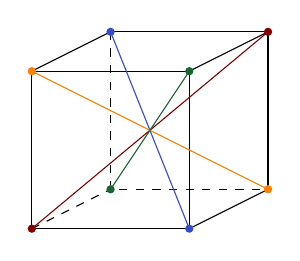
\begin{tikzpicture}
      \draw (0, 0) rectangle (2, 2);
      \draw (2, 0) -- +(1, 0.5);
      \draw (2, 2) -- +(1, 0.5);
      \draw (0, 2) -- +(1, 0.5);
      \draw [dashed] (0, 0) -- +(1, 0.5);
      \draw (1, 2.5) -- (3, 2.5) -- (3, 0.5);
      \draw [dashed] (1, 2.5) -- (1, 0.5) -- (3, 0.5);

      \draw [mred] (0, 0) node [circ] {} -- (3, 2.5) node [circ] {};
      \draw [mblue] (2, 0) node [circ] {} -- (1, 2.5) node [circ] {};
      \draw [morange] (0, 2) node [circ] {} -- (3, 0.5) node [circ] {};
      \draw [mgreen] (2, 2) node [circ] {} -- (1, 0.5) node [circ] {};
    \end{tikzpicture}
  \end{center}
  Then $G$ acts on $X$, and so we get $\phi: G \to \Sym(X)$. What is its kernel? To preserve the diagonals, it either does nothing, or flips the diagonals. So $G_X = \ker(\phi) = \{\id, \text{symmetry that sends each vertex to its opposite}\} \cong C_2$.

  How about the image? We have $G^X = \Im(\phi) \leq \Sym(X) \cong S_4$. It is an exercise to show that $\im(\phi) = \Sym(X)$, ie. it is surjective. We are not proving this because this is an exercise in geometry, not group theory. Then the first isomorphism theorem tells us
  \[
    G^X \cong G/G_X.
  \]
  So
  \[
    |G| = |G^X| |G_X| = 4! \cdot 2 = 48.
  \]
\end{eg}
This is an example of how we can use group actions to count elements in a group.

\begin{eg}[Cayley's theorem]
  For any group $G$, we have an action of $G$ on $G$ itself via
  \[
    g * g_1 = gg_1.
  \]
  It is trivial to check this is indeed an action. This gives a group homomorphism $\phi: G \to \Sym(G)$. What is its kernel? If $g \in \ker(\phi)$, then it acts trivially on every element. In particular, it acts trivially on the identity. So $g* e = e$, which means $g = e$. So $\ker(\phi) = \{e\}$. By the first isomorphism theorem, we get
  \[
    G \cong G/\{e\} \cong \im \phi \leq \Sym(G).
  \]
  So we know every group is (isomorphic to) a subgroup of a symmetric group.
\end{eg}

\begin{eg}
  Let $H$ be a subgroup of $G$, and $X = G/H$ be the set of left cosets of $H$. We let $G$ act on $X$ via
  \[
    g* g_1 H = gg_1 H.
  \]
  It is easy to check this is well-defined and is indeed a group action. So we get $\phi: G \to \Sym(X)$.

  Now consider $G_X = \ker(\phi)$. If $g \in G_X$, then for every $g_1 \in G$, we have $g * g_1 H = g_1H$. This means $g_1^{-1} gg_1 \in H$. In other words, we have
  \[
    g \in g_1 H g_1^{-1}.
  \]
  This has to happen for \emph{all} $g_1 \in G$. So
  \[
    G_X \subseteq \bigcap_{g_1 \in G} g_1 Hg_1^{-1}.
  \]
  This argument is completely reversible --- if $g \in \bigcap_{g_1 \in G} g_1 Hg_1^{-1}$, then
  \[
    g_1^{-1}g g_1 \in H,
  \]
  and hence
  \[
    gg_1 H = g_1H.
  \]
  So
  \[
    g* g_1 H = g_1 H
  \]
  for all $g_1 \in G$. So $g \in G_X$. Hence we indeed have equality:
  \[
    \ker (\phi) = G_X = \bigcap_{g_1 \in G} g_1 Hg_1^{-1}.
  \]
  Since this is a kernel, this is a normal subgroup of $G$, and is contained in $H$. Starting with an arbitrary subgroup $H$, this allows us to generate a normal subgroup, and this is indeed the biggest normal subgroup of $G$ that is in $H$, if we stare at it long enough.
\end{eg}

We can use this to prove the following theorem.
\begin{thm}
  Let $G$ be a finite group, and $H \leq G$ a subgroup of index $n$. Then there is a normal subgroup $K \lhd G$ with $K \leq H$ such that $G/K$ is isomorphic to a subgroup of $S_n$. Hence $|G/K| \mid n!$ and $|G/K| \geq n$.
\end{thm}

\begin{proof}
  We apply the previous example, giving $\phi: G \to \Sym(G/H)$, and let $K$ be the kernel of this homomorphism. We have already shown that $K \leq H$. Then the first isomorphism theorem gives
  \[
    G/K \cong \im \phi \leq \Sym(G/H) \cong S_n.
  \]
  The rest follows by Lagrange's theorem.
\end{proof}

\begin{cor}
  Let $G$ be a non-abelian simple group. Let $H \leq G$ be a subgroup of index $n > 1$. Then $G$ is isomorphic to a subgroup of $A_n$ with $n \geq 5$.
\end{cor}

\begin{proof}
  The action of $G$ on $X = G/H$ gives a homomorphism $\phi: G \to \Sym(X)$. Then $\ker(\phi) \lhd G$. Since $G$ is simple, $\ker(\phi)$ is either $G$ or $\{e\}$. We first show that it cannot be $G$. If $\ker(\phi) = G$, then every element of $G$ acts trivially on $X = G/H$. But if $g \in G\setminus H$, which exists since the index of $H$ is not $1$, then $g * H = gH \not= H$. So $g$ does not act trivially. So the kernel cannot be the whole of $G$. Hence $\ker(\phi) = \{e\}$.

  Thus by the first isomorphism theorem, we get
  \[
    G \cong \im (\phi) \leq \Sym(X) \cong S_n.
  \]
  We now need to show that $G$ is in fact a subgroup of $A_n$.

  Now $A_n \lhd S_n$. So $\im(\phi) \cap A_n \lhd \im(\phi) \cong G$. As $G$ is simple, $\im (\phi) \cap A_n$ is either $\{e\}$ or $G = \im(\phi)$. We want to show that the second thing happens, ie. the intersection is not the trivial group. We use the second isomorphism theorem. If $\im(\phi) \cap A_n = \{e\}$, then
  \[
    \im(\phi) \cong \frac{\im(\phi)}{\im(\phi) \cap A_n} \cong \frac{\im (\phi) A_n}{A_n} \leq \frac{S_n}{A_n} \cong C_2.
  \]
  So $G \cong \im (\phi)$ is a subgroup of $C_2$, ie. either $\{e\}$ or $C_2$ itself. Neither of these are non-abelian. So this cannot be the case. So we must have $\im(\phi) \cap A_n = \im(\phi)$, ie. $\im (\phi) \leq A_n$.

  The last part follows from the fact that $S_1, S_2, S_3, S_4$ have no non-abelian simple subgroups, which you can check by going to a quiet room and listing out all their subgroups.
\end{proof}

Let's recall some old definitions from IA Groups.
\begin{defi}[Orbit]
  If $G$ acts on a set $X$, the \emph{orbit} of $x \in X$ is
  \[
    G\cdot x = \{g * x \in X: g \in G\}.
  \]
\end{defi}

\begin{defi}[Stabilizer]
  If $G$ acts on a set $X$, the \emph{stabilizer} of $x \in X$ is
  \[
    G_x = \{g \in G: g * x = x\}.
  \]
\end{defi}

The main theorem about these concepts is the orbit-stabilizer theorem.
\begin{thm}[Orbit-stabilizer theorem]
  Let $G$ act on $X$. Then for any $x \in X$, there is a bijection between $G\cdot x$ and $G/G_x$, given by $g \cdot x \leftrightarrow g\cdot G_x$.

  In particular, if $G$ is finite, it follows that
  \[
    |G| = |G_x| |G \cdot X|.
  \]
\end{thm}
It takes some work to show this is well-defined and a bijection, but you've done it in IA Groups. In IA Groups, you probably learnt the second statement instead, but this result is more generally true for infinite groups.

\subsection{Conjugacy, centralizers and normalizers}
We have seen that every group acts on itself by multiplying on the left. A group $G$ can also act on itself in a different way, by conjugation:
\[
  g * g_1 = g g_1 g^{-1}.
\]
Let $\phi: G \to \Sym(G)$ be the associated permutation representation. Then
\[
  \phi(g) (g_1 \cdot g_2) = g g_1 g_2 g^{-1} = (g g_1 g^{-1})(g g_2 g^{-1}) = \phi(g)(g_1) \phi(g) (g_2).
\]
Thus we have shown that for each $g$, $\phi(g)$ is not just a map from $G$ to $G$, but a \emph{homomorphism} from $G$ to $G$. Since $\phi(g)$ is bijective (as in \emph{any} group action), it is in fact an isomorphism.

Thus, for any group $G$, there are many isomorphisms from $G$ to itself, one for every $g \in G$, and can be obtained from a group action of $G$ on itself.

Recall that at the beginning, we said groups are usually symmetries of some objects. Let's take a step further, and look at all symmetries of a group.
\begin{defi}[Automorphism group]
  The \emph{automorphism group} of $G$ is
  \[
    \Aut(G) = \{f: G \to G: f\text{ is a group isomorphism}\}.
  \]
  This is a group under composition, with the identity map as the identity.
\end{defi}
This is a subgroup of $\Sym(G)$, and the homomorphism $\phi: G\to \Sym(G)$ by conjugation lands in $\Aut(G)$.

This is pretty fun --- we can use this to cook up some more groups, by taking a group and looking at its automorphism group.

We can also take a group, take its automorphism group, and then take its automorphism group again, and do it again, and see if this process stabilizes, or becomes periodic.

\begin{defi}[Conjugacy class]
  The \emph{conjugacy class} of $g \in G$ is
  \[
    \ccl_G(g) = \{hgh^{-1}: h \in G\},
  \]
  ie. the orbit of $G \in G$ under the conjugation action.
\end{defi}

\begin{defi}[Centralizer]
  The \emph{centralizer} of $g \in G$ is
  \[
    C_G(g) = \{h \in G: hgh^{-1} = g\},
  \]
  ie. the stabilizer of $g$ under the conjugation action.
\end{defi}
This is alternatively the set of all $h \in G$ that commutes with $g$.

\begin{defi}[Center]
  The \emph{center} of a group $G$ is
  \[
    Z(G) = \{h \in G: hg h^{-1} = g\text{ for all }g \in G\} = \bigcap_{g \in G} C_G(g) = \ker (\phi).
  \]
\end{defi}
These are the elements of the group that commute with everything else.
\end{document}
